\documentclass[12pt]{article}

\setlength{\parindent}{0em}
\setlength{\parskip}{.5em}

\usepackage{framed}
\newcounter{problem}
\newcounter{problempart}[problem]
\newcounter{solutionpart}[problem]
\newenvironment{problem}{\stepcounter{problem}\noindent{\bf\arabic{problem}.}}{\setcounter{problempart}{0}\setcounter{solutionpart}{0}}
\newenvironment{solution}{\par\textcolor{blue}\bgroup}{\egroup\par}
\newcommand{\qpart}{\stepcounter{problempart}${}$\\\noindent{(\alph{problempart})} }
\newcommand{\spart}{\stepcounter{solutionpart}${}$\\\noindent{(\alph{solutionpart})} }
\newcommand{\TODO}{\textcolor{red}{$\blacksquare$}}
\newcommand{\SOL}[1]{\textcolor{blue}{#1}}

\usepackage{hyperref}
\usepackage{fullpage}
\usepackage{amsmath,mathabx,MnSymbol}
\usepackage{color,tikz}
\usepackage{footnote,enumitem}
\usepackage{longtable}
\newcommand{\mx}[1]{\begin{pmatrix}#1\end{pmatrix}}
\definecolor{dkgreen}{rgb}{0,.5,0}
\usepackage{algorithm}
\usepackage[noend]{algpseudocode}
\usetikzlibrary{calc}
\usetikzlibrary{decorations.pathreplacing}

\newcommand{\uu}{\mathbf{u}}
\newcommand{\vv}{\mathbf{v}}
\newcommand{\cc}{\mathbf{c}}
\newcommand{\ww}{\mathbf{w}}
\newcommand{\xx}{\mathbf{x}}
\newcommand{\zz}{\mathbf{z}}
\newcommand{\ee}{\mathbf{e}}
\newcommand{\pp}{\mathbf{p}}
\newcommand{\qq}{\mathbf{q}}
\renewcommand{\AA}{\mathbf{A}}
\newcommand{\BB}{\mathbf{B}}
\newcommand{\bb}{\mathbf{b}}
\renewcommand{\ss}{\mathbf{s}}
\newcommand{\CC}{\mathbf{C}}
\newcommand{\DD}{\mathbf{D}}
\newcommand{\dd}{\mathbf{d}}
\newcommand{\nn}{\mathbf{n}}
\newcommand{\gp}[1]{\left(#1\right)}

\newcommand{\TODOL}[1]{\textcolor{red}{\underline{\hspace{#1 cm}}}}

\usepackage{listings}

\lstset{
  language=C++,
  showstringspaces=false,
  identifierstyle=\color{magenta},
  basicstyle=\color{magenta},
  keywordstyle=\color{blue},
  identifierstyle=\color{black},
  commentstyle=\color{green},
  stringstyle=\color{red}
}

\begin{document}

\title{CS130 - Colors}
\date{}
\author{Name: \TODOL7\qquad\qquad SID: \TODOL4}
\maketitle
\begin{center}
\end{center}

\begin{problem}
  For each of the following RGB triples, identify the corresponding color.
  \begin{enumerate}[label=(\alph*)]
  \item $(0,0,0)$
  \item $(1,0,0)$
  \item $(0,1,0)$
  \item $(1,1,0)$
  \item $(0,0,1)$
  \item $(1,0,1)$
  \item $(0,1,1)$
  \item $(1,1,1)$
  \end{enumerate}
\end{problem}

\begin{problem}
  \newcommand{\h}{$\frac{1}{2}$}
  For each of the following colors, give an approximate RGB value for the color, where each of R,G,B is 0, $\frac{1}{2}$, or 1.  You must justify your answer.
  \begin{enumerate}[label=(\alph*)]
  \item gray
  \item pink
  \item navy blue
  \item orange
  \item forest green
  \item dark purple
  \item light green
  \end{enumerate}
\end{problem}

\begin{problem}
  Imagine that you have a fourth type of color sensitive cell in your eye that nobody else has.  (a) What would this allow you to do that others cannot?  (b) Devise an experiment that would allow you to convince others that you actually have this ability?
\end{problem}

\begin{solution}
  \textbf{\textcolor{red}{\TODO}}
\end{solution}

\section*{Ray tracing}

\begin{problem}
In the figure, you are given the position of the camera ($\ee$), the location of the center of the image plane ($\cc$), an up vector ($\ss$), and the width $w$ of the image plane (in 3D space).  You are also given the number of pixels in height and width ($H,W$) of the image.
\begin{center}
  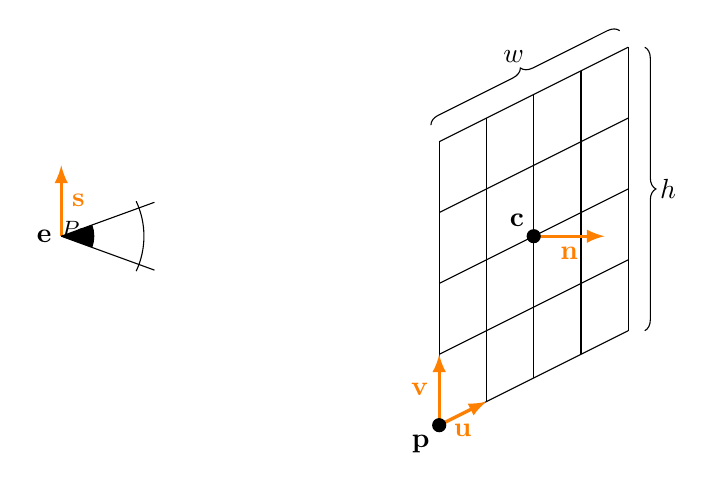
\begin{tikzpicture}[scale=3]
    \newcommand{\NP}{2}
    \newcommand{\PT}[2]{{2 + .2 * (#1) + 0 * (#2)},{0 + .1 * (#1) + .3 * (#2)}}
    \draw[-latex,orange,very thick](0,0)-- node[right]{$\ss$} ++ (0,.3);
    \draw[black] ([shift=(-25.000:0.350)]0.000,0.000) arc (-25.000:25.000:0.350);
    \draw[draw=none,fill=black] (0.000,0.000) -- ([shift=(-20.000:0.140)]0.000,0.000) arc (-20.000:20.000:0.140) -- cycle;
    \draw[black] (0.000,0.000) -- ++(-20.000:0.420);
    \draw[black] (0.000,0.000) -- ++(20.000:0.420);
    \foreach \i in {-\NP,...,\NP}
    {
      \draw[](\PT{\i}{-\NP})--(\PT{\i}{\NP});
      \draw[](\PT{-\NP}{\i})--(\PT{\NP}{\i});
    }
    \draw[-latex,orange,very thick](\PT{-\NP}{-\NP})-- node[below]{$\uu$} (\PT{1-\NP}{-\NP});
    \draw[-latex,orange,very thick](\PT{-\NP}{-\NP})-- node[left]{$\vv$} (\PT{-\NP}{1-\NP});
    \draw[draw=none,fill=black](\PT{-\NP}{-\NP}) circle (.03) node[below left]{$\pp$};
    \draw[-latex,orange,very thick](\PT{0}{0})-- node[below]{$\nn$} ++ (.3,0);
    \draw[draw=none,fill=black](\PT{0}{0}) circle (.03) node[above left]{$\cc$};
    \node[left] at (0,0) {$\ee$};
    \draw [decorate,decoration={brace,amplitude=4pt},xshift=2pt,yshift=0pt] (\PT{\NP}{\NP}) -- node[right,xshift=2pt]{$h$} (\PT{\NP}{-\NP});
    \draw [decorate,decoration={brace,amplitude=4pt},xshift=-1pt,yshift=2pt] (\PT{-\NP}{\NP}) -- node[above left,yshift=2pt,xshift=3pt]{$w$} (\PT{\NP}{\NP});
{\footnotesize $P_1$};
  \end{tikzpicture}
\end{center}
  Determine the height $h_p$ and width $w_p$ of a pixel.  You may assume that the pixels are squares.
\end{problem}

\begin{solution}
  \textbf{\textcolor{red}{\TODO}}
\end{solution}

\begin{problem}
Compute the height $h$ of the image plane (in 3D space).
\end{problem}

\begin{solution}
  \textbf{\textcolor{red}{\TODO}}
\end{solution}

\begin{problem}
  The ray from $\ee$ to $\cc$ is assumed to be orthogonal to the image plane.  Find the plane's normal $\nn$.
\end{problem}

\begin{solution}
  \textbf{\textcolor{red}{\TODO}}
\end{solution}

\begin{problem}
  The up vector $\ss$ we are given need not be orthogonal to $\nn$, so we cannot use it as our image's up vector $\vv$.  Instead, we must first compute $\hat\uu$ orthogonal to $\nn$ and $\ss$.  Then, we can compute $\hat\vv$ from $\nn$ and $\hat\uu$.  Both $\hat\uu$ and $\hat\vv$ should be normalized.  If we are standing at $\ee$ and looking at $\cc$ with $\ss$ pointing roughly upwards, then $\hat\uu$ should be pointing to the right, and $\hat\vv$ should be pointing upwards.  Make sure you check that these two vectors point in the correct direction.  Don't worry about their length yet.
\end{problem}

\begin{solution}
  \textbf{\textcolor{red}{\TODO}}
\end{solution}

\begin{problem}
  Next, we scale $\hat\uu$ to $\uu$ and $\hat\vv$ to $\vv$ so that $\|\uu\| = w_p$ and $\|\vv\| = h_p$.  In this way, adding $\uu$ causes us to move right one pixel, and adding $\vv$ causes us to move up one pixel.
\end{problem}

\begin{solution}
  \textbf{\textcolor{red}{\TODO}}
\end{solution}

\begin{problem}
  Find the bottom left corner $\pp$.
\end{problem}

\begin{solution}
  \textbf{\textcolor{red}{\TODO}}
\end{solution}

\begin{problem}
  Given a pixel index $(i,j)$, find the corresponding point $\xx$ on the image plane.  Note that pixel index $(i,j)$ refers to the \textit{center} of pixel $(i,j)$, with pixel $(0,0)$ being the bottom left pixel and $(W-1,H-1)$ being the top right pixel.  Note that $\pp$ is at the corner of the image, not the center of the lower left pixel.
\end{problem}

\begin{solution}
  \textbf{\textcolor{red}{\TODO}}
\end{solution}

\begin{problem}
  Find the endpoint and (normalized) direction of the ray that should be cast through pixel $(i,j)$.
\end{problem}

\begin{solution}
  \textbf{\textcolor{red}{\TODO}}
\end{solution}


\end{document}
